\section{Data Description}

\subsection{Prices, Exchanges, and Coin characteristics}


%\begin{figure}[h]
%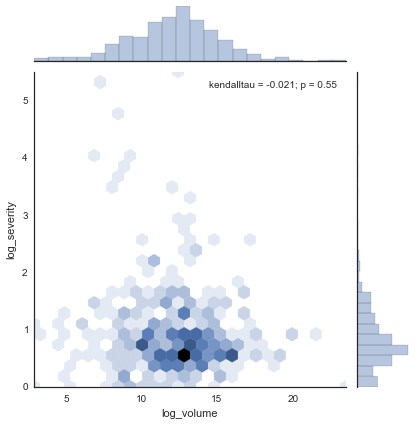
\includegraphics[width=\columnwidth]{severity_volume}
%\end{figure}

Our main outcome measures are the severity of drop in the value of a unit of the asset, and the magnitude in USD of the transactions in them.
To obtain data for them we scrape three market aggregators. 

We operationalize the intensity of a bubble as the proportion of a 1 dollar that would be lost buying at the maximum price and selling after that proportionally to the volume of the market till the present, we call this severity.

We define the volume as the sum of the contemporaneous dollar (todo check) volume of trade.

As a secondary outcome measure we consider the number of exchanges that list the coin.
